\documentclass[tikz,border=10pt]{standalone}
\usepackage{tikz}
\usetikzlibrary{positioning,arrows.meta,shapes,calc}

\begin{document}
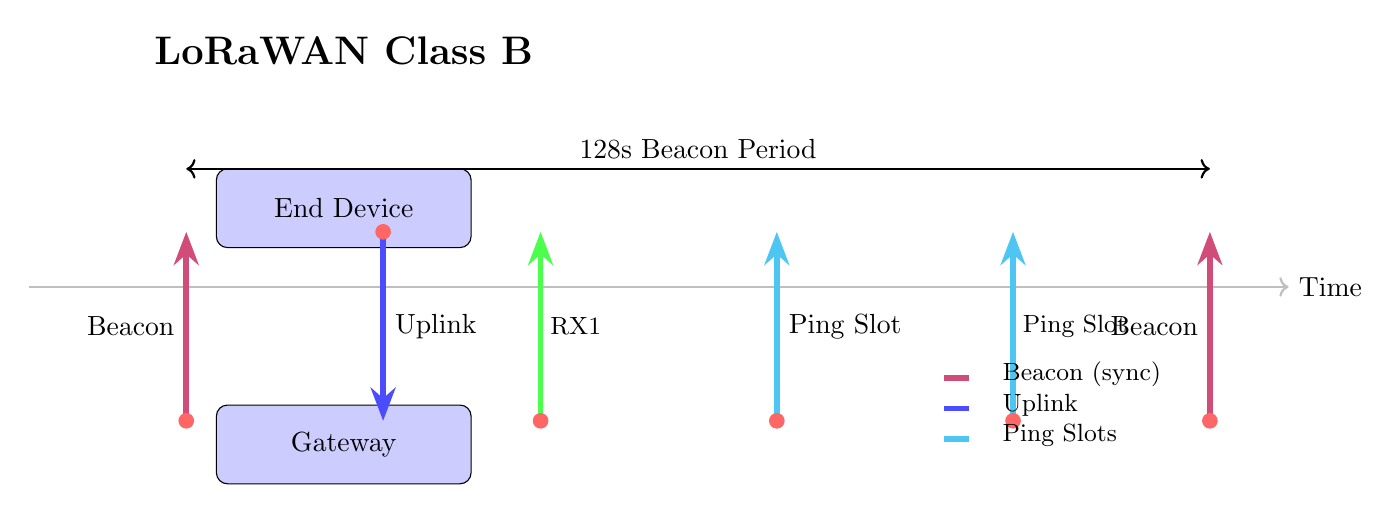
\begin{tikzpicture}[
    node distance=1.5cm,
    block/.style={rectangle, draw, fill=blue!20, text width=3cm, text centered, rounded corners, minimum height=1cm},
    arrow/.style={-Stealth, thick},
    timeline/.style={->, thick, draw=gray!50},
    event/.style={circle, fill=red!60, inner sep=2pt}
]

% Title
\node[font=\Large\bfseries] at (0,5) {LoRaWAN Class B};

% Device
\node[block] (device) at (0,3) {End Device};

% Gateway
\node[block] (gateway) at (0,0) {Gateway};

% Timeline
\draw[timeline] (-4,2) -- (12,2) node[right] {Time};

% Beacon
\draw[arrow, purple!70, line width=2pt] (-2,0.3) -- node[left, black] {Beacon} (-2,2.7);
\node[event] at (-2,0.3) {};

% Uplink
\draw[arrow, blue!70, line width=2pt] (0.5,2.7) -- node[right, black] {Uplink} (0.5,0.3);
\node[event] at (0.5,2.7) {};

% RX1
\draw[arrow, green!70, line width=2pt] (2.5,0.3) -- (2.5,2.7);
\node[event] at (2.5,0.3) {};
\node[right] at (2.5,1.5) {\small RX1};

% Ping Slot
\draw[arrow, cyan!70, line width=2pt] (5.5,0.3) -- node[right, black] {Ping Slot} (5.5,2.7);
\node[event] at (5.5,0.3) {};

% Another Ping Slot
\draw[arrow, cyan!70, line width=2pt] (8.5,0.3) -- (8.5,2.7);
\node[event] at (8.5,0.3) {};
\node[right] at (8.5,1.5) {\small Ping Slot};

% Next Beacon
\draw[arrow, purple!70, line width=2pt] (11,0.3) -- node[left, black] {Beacon} (11,2.7);
\node[event] at (11,0.3) {};

% Beacon period indicator
\draw[<->, thick] (-2,3.5) -- (11,3.5) node[midway, above] {128s Beacon Period};

% Legend
\node[font=\small] at (9,0.5) {
    \begin{tabular}{ll}
    \textcolor{purple!70}{\rule{1em}{2pt}} & Beacon (sync) \\
    \textcolor{blue!70}{\rule{1em}{2pt}} & Uplink \\
    \textcolor{cyan!70}{\rule{1em}{2pt}} & Ping Slots \\
    \end{tabular}
};

\end{tikzpicture}
\end{document}
